% % % % % % %
%  Packages %
% % % % % % %

%---Base packages
\documentclass[a4paper,12pt,oneside]{report}	% document type (article, report, book)
\usepackage[utf8]{inputenc}			% encoding
\usepackage[T1]{fontenc}			% accent
\usepackage{lmodern}				% latin font
\usepackage{appendix}				% to be able to use appendices
\usepackage{tabularray}

%---Language(s)
\usepackage[english,frenchb]{babel}	% last language = typography by default
\addto\captionsfrench{				% to change the french names of...}
	\renewcommand{\appendixpagename}{Annexes}	% (default Appendices)
	\renewcommand{\appendixtocname}{Annexes}	% (default Appendices)
	\renewcommand{\tablename}{\textsc{Tableau}}	% (default \textsc{Table})
}

%---Page layout
%------> margins
	% 1st option -> geometry package
		%\usepackage[a4paper]{geometry}		% default parameters for A4
		%\usepackage[top=2in, bottom=1.5in, left=1in, right=1in]{geometry}
	% 2nd option -> a4wide package
		\usepackage{a4wide}		% A4 with smaller margins (the one I've chosen)
	% 3rd option -> fullpage package
		%\usepackage{fullpage}
%------> chapter style
	% 1st option -> fncychap package
		%\usepackage[style]{fncychap}		% style = Lenny, Bjornstrup, Sonny, Conny
	% 2nd option -> customized styles
		%
%------> cover page (UMONS template)
	\usepackage[fpms]{umons-coverpage}		% NEED "umons-coverpage.sty" file
	\umonsAuthor{Noms des auteurs : exemple \\ Théo \textsc{Dupont}}
	\umonsTitle{Titre du rapport}
	\umonsSubtitle{Sous-titre du rapport}
	\umonsDocumentType{Type de document}
	\umonsSupervisor{Sous la direction de : \\ Prof. T.\textsc{DUPONT} \\ Assistant T.\textsc{DUPOND}}
	\umonsDate{Date du rapport}

%---Numbering
\setcounter{secnumdepth}{2}			% numerotation depth (1=sec and all above)
\setcounter{tocdepth}{2}			% table of contents depth (1=sec and above)

%---Mathematics
\usepackage{amsmath}				% base package for mathematics
\usepackage{amsfonts}				% base package for mathematics
\usepackage{amssymb}				% base package for mathematics
%\usepackage{amsthm}				% theorem and proof environments
%\usepackage{cases}					% numcases environment
%\usepackage{mathrsfs}				% \mathscf command ('L' of Laplace-Transform,...)

%---Floating objects (images, tables,...)
\usepackage{float}					% better management of floating objects
\usepackage{array}					% better management of tables
\usepackage{graphicx}				% to include external images
\usepackage{wrapfig}
\graphicspath{ {./figures/} } 
%\usepackage{caption}				% /!\ has priority on "memoir" class
%\usepackage{subcaption}			% subfigure and subtable environments
%\usepackage{subfig}				% \subfloat command
%\usepackage{wrapfig}				% wrapfigure environment
%\usepackage[update]{epstopdf}		% to use '.eps' files with PDFLaTeX

%---Code including
\usepackage{listings}				% general package (can be tuned)
\usepackage{caption}
\newenvironment{code}{\captionsetup{type=listing}}{}
\usepackage[newfloat]{minted}
\usepackage{color}
%\usepackage[framed]{mcode}			% to include Matlab code
									% /!\ you need the "mcode.sty" file

%---Units from International System
\usepackage{siunitx}				% \SI{}{} command (units with good typography)
\DeclareSIUnit\baud{baud}			% definition of the "baud" unit
\DeclareSIUnit\bit{bit}				% definition of the "bit" unit

%---Drawing
\usepackage{tikz}					% useful package for drawing
\usepackage[european]{circuitikz} 	% to draw electrical circuits

%---Bibliography
\usepackage{url}					% to encore url
\usepackage[style=numeric-comp,backend=bibtex]{biblatex}
\usepackage{csquotes}				% inverted commas in references
\bibliography{bibli}				% your .bib file

%---"hyperref" package				% /!\ it must be the last package
\usepackage[hidelinks]{hyperref}	% clickable links (table of contents,...)
\hypersetup{
    colorlinks,
    citecolor=black,
    filecolor=black,
    linkcolor=black,
    urlcolor=black
}

% % % % % % %
% Document	%
% % % % % % %

\begin{document}
% Ask for a regular cover page with full content and default picture
\umonsCoverPage 
\pagenumbering{roman}

\begin{abstract}    %Résumé%  
	...
\end{abstract}

\renewcommand{\abstractname}{Remerciements}     %Remerciements%
\begin{abstract}
     ...
\end{abstract}

\clearpage
\tableofcontents    %Table des matières%

\clearpage
\pagenumbering{arabic}
% Start your document ...

\chapter*{Introduction}
\addcontentsline{toc}{chapter}{Introduction}
    \section*{partie 1 intro}
    \addcontentsline{toc}{section}{partie 1 intro}


\chapter{Exemples}

\section{Exemple figure}

\begin{figure}[H]
    \centering
    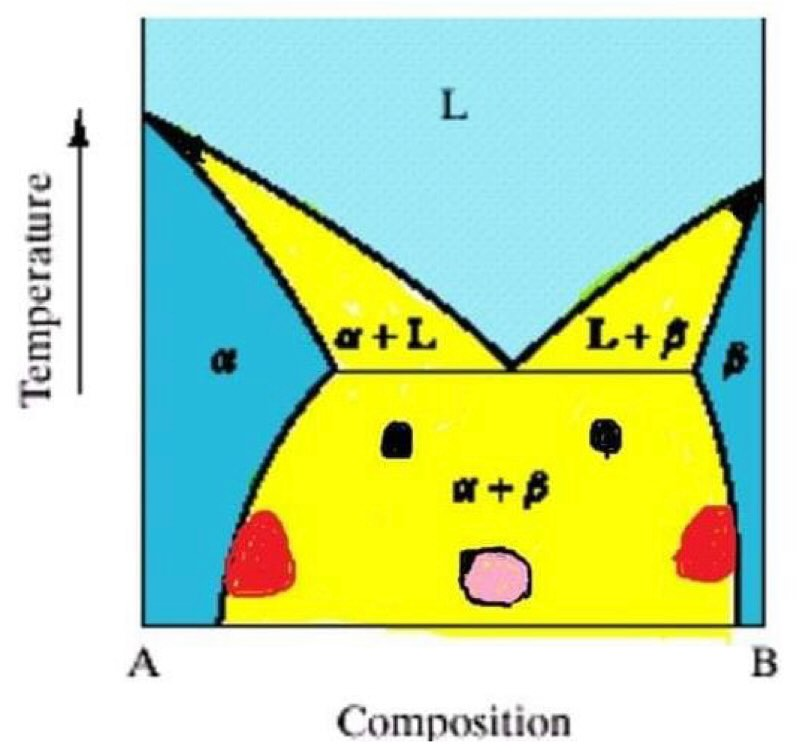
\includegraphics[width=0.5\linewidth]{figures/pikachu.jpg}
    \caption{Figure exemple}
    \label{fig exemple}
\end{figure}


\section{Exemple tableau}

\begin{table}[H]
    \centering
    \begin{tabular}{c|c|c}
    $I_{U}[A]$ & $U_{1L} [V]$ & $g$ \\ \hline
       &   &   \\
       &   &   \\
       &   &   \\
       &   &   \\
       &   &   \\
       &   &   \\
       &   &   \\
       &   &   \\
       &   &   \\
       &   &   \\
       &   &   \\
       &   &   \\
       &   &   \\
       &   &   \\
       &   &   \\
    \end{tabular}
    \caption{Tableau exemple}
    \label{tab exemple}
\end{table}

\section{Exemple équation}

\begin{equation}
    I_C-I_{1m}+I_g\cdot sin(\varphi)=0
    \label{éq exemple}
\end{equation}

\section{Exemple code}

\begin{figure}[H]
    \centering
    \begin{minted}[frame=single, framesep=10pt, mathescape, linenos]{php}
    <?php
    if (isset($_POST['delete'])) {
        $user_id = $_SESSION['ID'];

        $sql = "DELETE FROM tableau WHERE ID='$user_id'";
        if (mysqli_query($conn, $sql)) {
        } else {
            echo "Erreur : " . mysqli_error($conn);
        }
    }
    ?>
    \end{minted}
    \caption{Code exemple}
    \label{code exemple}
\end{figure}

\chapter*{Conclusion}
\addcontentsline{toc}{chapter}{Conclusion}	% to add in the toc

% Appendices
\clearpage
\pagenumbering{gobble} %pas de numérotation de page
\appendix		% Changes the numbering of chapters to an alphabetic form and
				% also changes the names of chapters from \chaptername 
				% to the value of \appendixname.
%\addappheadtotoc*% Makes an entry in the ToC
\appendixpage	% Generates a part-like page with the title given by
				% the value of \appendixpagename. 
	
\chapter*{Annexe 1}

% Bibliography
	%\clearpage			% if it does'nt start on a new page
	%\phantomsection	% if any problem with the reference in the toc
\printbibliography
%\addcontentsline{toc}{chapter}{Bibliographie}

\end{document}

